\centering
\large\sffamily
\tikzstyle{box}=[draw, thick, rectangle, inner sep=0pt, minimum width=1cm, minimum height=1cm, anchor=south west]
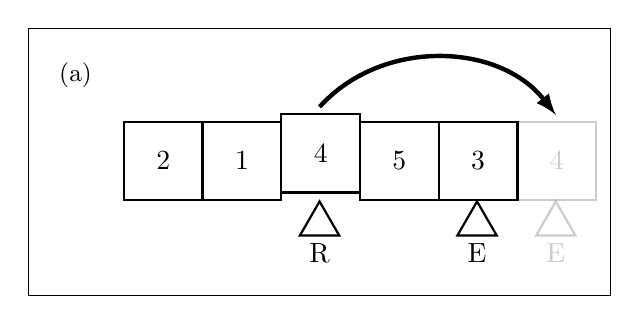
\begin{tikzpicture}
	\draw (-1.2, -1.2) rectangle (6.2, 2.2);
	\node at (-.6, 1.6) {\small(a)};
	\node[box] at (0, 0) {2};
	\node[box] at (1, 0) {1};
	\node[box] at (2, .1) {4};
	\node[box] at (3, 0) {5};
	\node[box] at (4, 0) {3};
	\node[box, opacity=.2] at (5, 0) {4};
	\draw[thick] (2.5, 0) -- ++(-60:.5) -- ++(180:.5) -- cycle node[below=4mm] {R};
	\draw[thick] (4.5, 0) -- ++(-60:.5) -- ++(180:.5) -- cycle node[below=4mm] {E};
	\draw[thick, opacity=.2] (5.5, 0) -- ++(-60:.5) -- ++(180:.5) -- cycle node[below=4mm] {E};
	\path[-{latex}, ultra thick] (2.5, 1.2) edge[bend left=50] (5.5, 1.1);
\end{tikzpicture}
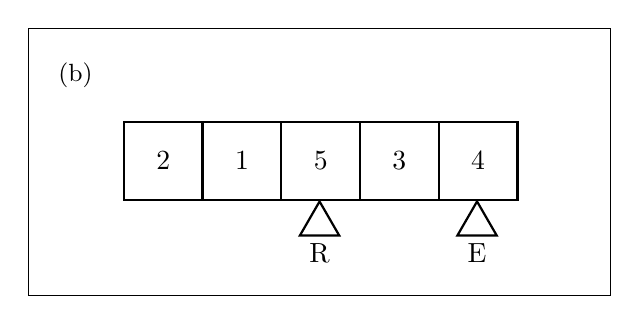
\begin{tikzpicture}
	\draw (-1.2, -1.2) rectangle (6.2, 2.2);
	\node at (-.6, 1.6) {\small(b)};
	\node[box] at (0, 0) {2};
	\node[box] at (1, 0) {1};
	\node[box] at (2, 0) {5};
	\node[box] at (3, 0) {3};
	\node[box] at (4, 0) {4};
	\draw[thick] (2.5, 0) -- ++(-60:.5) -- ++(180:.5) -- cycle node[below=4mm] {R};
	\draw[thick] (4.5, 0) -- ++(-60:.5) -- ++(180:.5) -- cycle node[below=4mm] {E};
\end{tikzpicture}\par\vspace{1mm}%
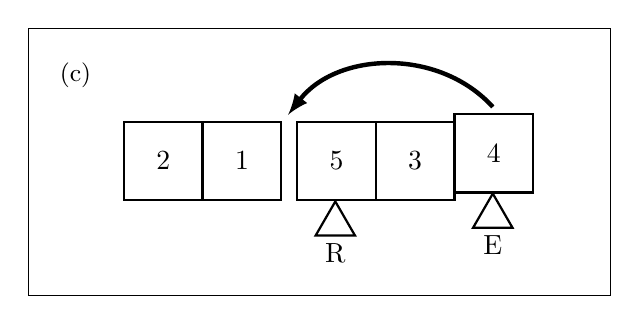
\begin{tikzpicture}
	\draw (-1.2, -1.2) rectangle (6.2, 2.2);
	\node at (-.6, 1.6) {\small(c)};
	\node[box] at (0, 0) {2};
	\node[box] at (1, 0) {1};
	\node[box] at (2.2, 0) {5};
	\node[box] at (3.2, 0) {3};
	\node[box] at (4.2, 0.1) {4};
	\draw[thick] (2.7, 0) -- ++(-60:.5) -- ++(180:.5) -- cycle node[below=4mm] {R};
	\draw[thick] (4.7, .1) -- ++(-60:.5) -- ++(180:.5) -- cycle node[below=4mm] {E};
	\path[-{latex}, ultra thick] (4.7, 1.2) edge[bend right=50] (2.1, 1.1);
\end{tikzpicture}
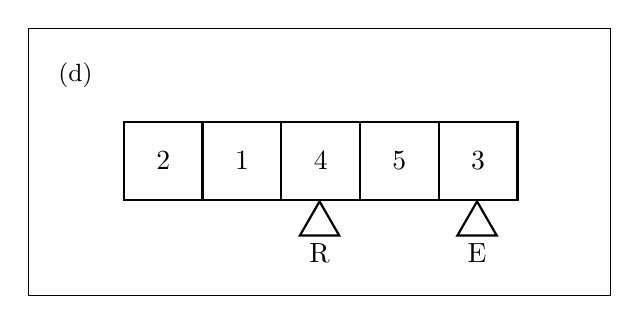
\begin{tikzpicture}
	\draw (-1.2, -1.2) rectangle (6.2, 2.2);
	\node at (-.6, 1.6) {\small(d)};
	\node[box] at (0, 0) {2};
	\node[box] at (1, 0) {1};
	\node[box] at (2, 0) {4};
	\node[box] at (3, 0) {5};
	\node[box] at (4, 0) {3};
	\draw[thick] (2.5, 0) -- ++(-60:.5) -- ++(180:.5) -- cycle node[below=4mm] {R};
	\draw[thick] (4.5, 0) -- ++(-60:.5) -- ++(180:.5) -- cycle node[below=4mm] {E};
\end{tikzpicture}